\section{实验分析}
\label{evaluation}

\subsection{单日数据预测第二天采食量}

本节训练模型使用的数据每条样本格式为
\begin{equation}
\label{sample}
	\langle (y_t, m_t, T^h_t), y_{t+1} \rangle
\end{equation}
	其中输入变量$y_t$为第$t$天某牛棚的头均采食量,$m_t$为第$t$天头均产奶量,$T_t^h$为第$t$天的最高气温,输出变量(预测值)$y_{t+1}$为第$t+1$天的头均采食量。
经过数据预处理,得到数据样本约1750条。
	
在部分实验中我们采用了\emph{对照组},对照组作为比较的基准对象用最简易傻瓜的方式建模预测,具体地,$\hat y_{t+1} = y_t$,即用当天的实际头均采食量直接作为第二天的头均采食量预测值。

	
\subsubsection{模拟对历史数据的拟合}

XGBoost模型拟合历史数据的平均绝对误差请见表\ref{tab:singleday_all},部分样本的预测值和实际值请见图\ref{fig:singleday_all}。XGBoostost模型的参数n\_estimators取200,max\_depth取2(参见第\ref{best_para}节)。

表\ref{tab:singleday_all}显示单日数据构建的模型相比于对照组能够有效减小平均绝对误差MAE,$\epsilon_{MAE}=1.01$指每日预测头均和实际头均的平均绝对误差是1.01千克,平均误差率约在$2.5\%\sim3.4\%$左右。$R^2$刻划模型对数据的拟合度,0.886意味着拟合度很高,模型对历史数据拟合能力强。

\begin{table}
\caption{单日数据建模拟合历史数据的误差。}
\begin{center}
\footnotesize
\begin{tabular}{|c|c|}
\hline
	指标 & 值\\
\hline
	$\epsilon_{MAE}$  &  1.01\\
	对照组$\epsilon_{MAE}$ & 1.274 \\
	$R^2$  &  0.886 \\
\hline
\end{tabular}
\end{center}
\label{tab:singleday_all}
\end{table}

\begin{figure}
\begin{center}
	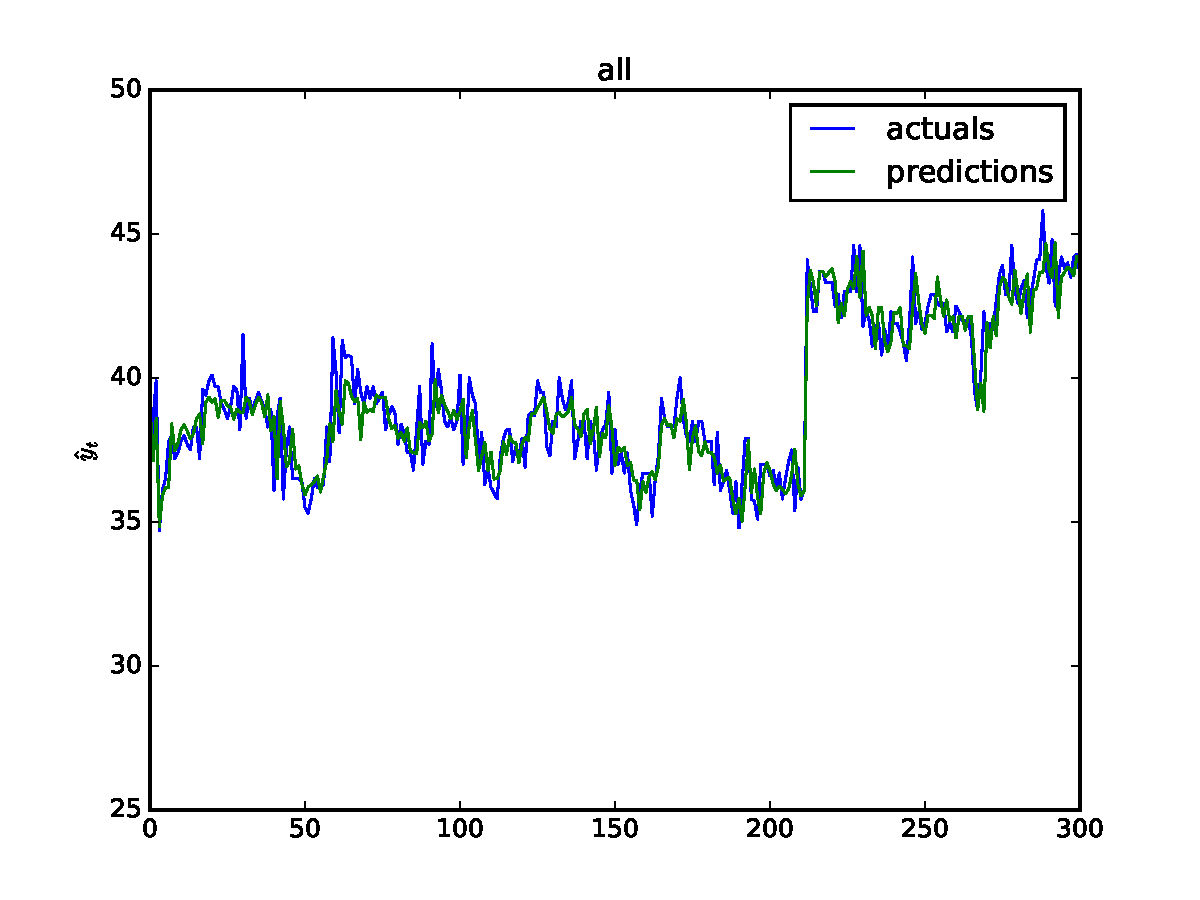
\includegraphics[width=0.9\linewidth]{singleday_all}
\caption{单日数据建模在部分样本上的预测结果。}
\label{fig:singleday_all}
\end{center}
\end{figure}

另外通过XGBoost的plot\_importance函数可以可视化不同特征对于模型的重要性或贡献程度,结果如图\ref{fig:feature_importance}所示。由图可知,当取单日观测数据拟合第二天头均采食量时,各特征重要性排序为:头均采食量>头均产奶量>最高气温。

\begin{figure}
\begin{center}
	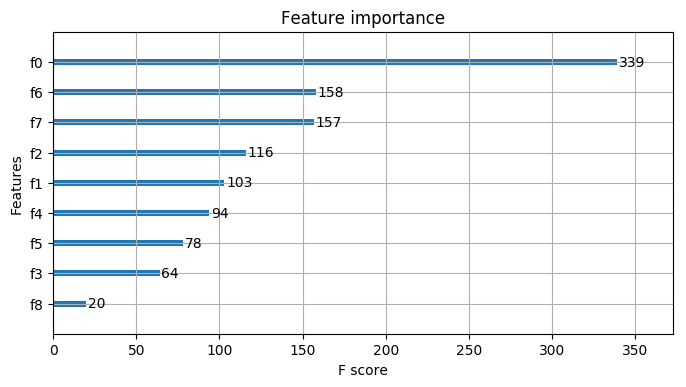
\includegraphics[width=0.9\linewidth]{feature_importance}
\caption{不同特征对XGBoost模型的贡献程度。$f0,f1,f2$分别对应数据样本中的$y_t, m_t, T^h_t$。}
\label{fig:feature_importance}
\end{center}
\end{figure}

模型对历史数据的拟合只能说明模型复杂程度足够高,但不能说明模型对于\uline{未见过的数据样本}具有较强的预测能力,即对于有预测性质的任务,我们更需要关注模型的\emph{泛化能力}。
我们在下一小节做相关分析。

\subsubsection{模拟对未见数据的预测}
\label{predict_singleday}

我们采用交叉验证\footnote{具体地,$k$折交叉验证将所有数据样本随机平均分为$k$组,重复$k$次测试:每次测试用其中$k-1$组数据样本组合成训练集,训练构建得到模型(预测器),并将模型用于剩下的一组数据样本(作为测试集)进行预测,并在测试集上评估相关误差指标。}的方式评估模型的泛化能力,即对历史未见数据的预测能力。


\begin{table}
\caption{单日数据建预测时5折交叉验证的误差。}
\begin{center}
\footnotesize
\begin{tabular}{|c|c|}
\hline
	$\epsilon_{MAE}$ & $R^2$ \\
\hline
 1.202 &  0.728\\
 1.221 &  0.797\\
 1.243 &  0.744 \\
 1.359 &  0.724 \\
 1.430 &  0.560 \\
\hline
\end{tabular}
\end{center}
\label{tab:singleday_predict_all}
\end{table}


表\ref{tab:singleday_predict_all}显示了对所有数据样本做5折交叉验证的结果(交叉验证时不同随机分组会导致不同的结果,表中显示随机挑选某次实验的结果)。
比较表\ref{tab:singleday_predict_all}和\ref{tab:singleday_all},可知预测时的平均$\epsilon_{MAE}=1.291$略高于对照组的$\epsilon_{MAE}$,模型相比于对照组\uline{预测失效}。
虽然在上一节观察到模型拟合历史数据的能力较强,但交叉验证的结果说明模型缺乏泛化能力,这主要由两个可能原因导致:(1)在部分实验中$\epsilon_{MAE}$较高,原因可能是在拆分训练集和测试集时,某些相对难预测的模式的样本被分至测试集但未出现在训练集中(导致模型未能学到这些模式)。
如数据集规模进一步增大,则模型的预测性能应当进一步提升。
(2)仅以单日观测数据作为特征,缺乏对采食量变化模式的刻划能力。我们在第\ref{temporal}节尝试改进措施。



\subsubsection{分牛棚的拟合和预测分析}
\label{predict_singleday_cowshed}

我们进一步分析模型对于不同牛棚的牛群采食量的预测能力。
我们先用所有样本数据训练得到模型去\emph{拟合}各个牛棚的数据,观察模型对于不同牛棚牛群采食量刻划效果的差异,结果如表\ref{tab:regression_multicowshed}所示。

\begin{table}
\caption{不同牛棚头均采食量拟合的误差。}
\begin{center}
\footnotesize
\begin{tabular}{|c|c|c|c|c|}
\hline
	牛棚 & 牛只类型 & $\epsilon_{MAE}$ & 对照组$\epsilon_{MAE}$ &$R^2$ \\
\hline
B1-1N& 头胎 & 0.793 & 0.964 & 0.424 \\
B1-1S& 头胎 & 0.657 & 0.865 & 0.73 \\
B1-3N& 多胎 & 0.756 & 0.751 & 0.475 \\
B1-3S& 头胎 & 0.706 & 0.726 & 0.696 \\
B1-5N& 头胎 & 1.173 & 1.824 & 0.846 \\
B1-5S& 头胎 & 1.375 & 2.806 & 0.919 \\
B1-7N& 头胎 & 1.232 & 1.477 & 0.898 \\
B1-7S& 多胎 & 0.995 & 1.105 & 0.458 \\
B4-1N& 参配 & 1.095 & 1.56 & 0.584 \\
B4-1S& 怀孕 & 0.969 & 1.193 & 0.699 \\
B4-3N& 蹄病 & 1.248 & 1.455 & 0.501 \\
B4-3S& 高产 & 1.39 & 1.743 & 0.564 \\
B4-5N& 多胎 & 0.882 & 1.197 & 0.757 \\
B4-5S& 头胎 & 1.008 & 1.088 & 0.556 \\
B4-7N& 多胎 & 1.071 & 1.192 & 0.664 \\
B4-7S& 头胎 & 0.913 & 0.987 & 0.798 \\
\hline
\end{tabular}
\end{center}
\label{tab:regression_multicowshed}
\end{table}

观察可以发现(1)各牛棚模型拟合平均绝对误差均低于对照组;
(2)不同牛棚拟合的误差有高有低,大致和对照组拟合误差高低趋势一致。
观察(2)说明模型的预测误差主要来自于日头均采食量的较大波动,而模型难以预测这种突然的升、降。
$R^2$值最高的(模型拟合度最高的)几个牛棚为B1-5S、B1-7N、B1-5N、B4-7S、B4-5S($R^2$均高于0.75)。
这些牛棚除B4-5S外,均为“头胎”,其原因可能是“头胎”牛占数据样本中的大多数,使得模型对于该类型牛的采食量模式刻划得较好。而牛只这也说明不同类型牛的采食量模式存在差异。
因而在建模时应当考虑如下权衡:

\emph{问题:建模时应对不同品种、类型(头胎、多胎、参配等)的牛群分别构建模型,还是用同一模型建模,用某些特征来表征这种差异?}

如果数据量充足,且能够提取富有表征能力的特征,则构建统一模型可以达到较好的预测效果(有待未来实验验证)。

但当前训练数据样本有限且特征不够丰富,我们先尝试简化问题进行分牛棚的实验:排除影响模型预测效果的因素,只选取牛只类别为“头胎”的牛棚,单独进行建模。
如此筛选得到约760条数据样本,在所有“头胎”牛棚牛群上进行5折交叉验证,实验结果如表\ref{tab:singleday_first_predict_all}所示。在只考虑“头胎”牛群时,对照组的平均绝对误差$\epsilon_{MAE}$为1.306。观察表格结果可见5折交叉验证的$\epsilon_{MAE}$的平均值1.328高于对照组,且高于不区分牛群时的平均$\epsilon_{MAE}$,说明模型\uline{预测失效}。原因如第\ref{predict_singleday}节所述,主要有二:(1)数据量过小,测试集中存在训练集未涵盖的采食量变化模式,导致模型泛化能力差;(2)模型的输入变量缺乏富有表征力的特征。
其中原因(1)尤为重要,因为如只选择“头胎”牛群,则数据集样本数仅为约760,不到上节全部牛群数据量的一半。

\begin{table}
\caption{单日数据建预测“头胎”牛群时5折交叉验证的误差。}
\begin{center}
\footnotesize
\begin{tabular}{|c|c|}
\hline
	$\epsilon_{MAE}$ & $R^2$ \\
\hline
  1.361  &  0.627 \\
 1.404  &  0.560 \\
 1.231  &  0.750 \\
 1.376  &  0.720 \\
 1.267  &  0.653 \\
\hline
\end{tabular}
\end{center}
\label{tab:singleday_first_predict_all}
\end{table}




\subsection{加入时域信息预测第二天采食量}
\label{temporal}

\begin{figure}
\begin{center}
	\includegraphics[width=0.8\linewidth]{feature_importance_gradient}
\caption{不同特征对XGBoost模型的贡献程度。$f0,f1,f2,f3$分别对应数据样本中的$y_t, m_t, T^h_t, g_{t,k}$。}
\label{fig:feature_importance_gradient}
\end{center}
\end{figure}

本节训练模型使用的数据每条样本格式为:
\begin{equation}
	\langle (y_t, m_t, T^h_t, g_{t,k}), y_{t+1} \rangle
\end{equation}
相比于式\ref{sample}新增了一项$g_{t,k}$,表示从第$t$天开始向前回溯$k$天的采食量的梯度值。
具体地,$g_{t,k}$是用线性回归拟合点集$\{(1, y_{t-k+1}), (2, y_{t-k+2}), \cdots, (k, y_{t})\}$得到直线的斜率。我们希望引入该项来增加刻划时域上头均采食量变化趋势的特征。

我们设定$k=3$(考虑过去3天采食量的梯度),经过数据预处理、缺失值剔除,得到全部数据样本约1700条。实验中XGBoost模型的参数n\_estimators取150,max\_depth取2(参见第\ref{best_para}节)。
在所有数据样本做拟合分析各特征的重要性,结果如图\ref{fig:feature_importance_gradient}所示。
由图可知,当引入时域特征拟合第二天头均采食量时,各特征重要性排序为:头均采食量>头均产奶量>最高气温 $\approx$ 头均采食量时域梯度。


对所有数据样本做5折交叉验证的结果如表\ref{tab:gradient_predict_all}所示。
对照组(用当天头均采食量直接当做第二天头均采食量预测值)的$\epsilon_{MAE}$为1.274。分析表格可见$\epsilon_{MAE}$的平均值1.209低于对照组,说明\uline{预测有效},虽然改进并不显著。

\begin{table}
\caption{加入时域信息预测所有牛群时5折交叉验证的误差。}
\begin{center}
\footnotesize
\begin{tabular}{|c|c|}
\hline
	$\epsilon_{MAE}$ & $R^2$ \\
\hline
1.239 & 0.767 \\
1.193 & 0.772 \\
1.203 & 0.768 \\
1.196 & 0.822 \\
1.215 & 0.706 \\
\hline
\end{tabular}
\end{center}
\label{tab:gradient_predict_all}
\end{table}

我们仿照第\ref{predict_singleday_cowshed}节,剔除其他类别的牛群,仅对“头胎”牛群进行分析,则结果和第\ref{predict_singleday_cowshed}节类似,预测误差1.286高于对照组1.258,且高于不拆分牛群的预测结果(1.209)。数据集样本量不够大是主要原因。


